\chapter{Reinforcement Learning}
\epigraph{
  Fool me once, shame on you \\
  fool me twice, shame on me.
}{Popular proverb}


\section{The Problem}
Reinforcement Learning in general is
the idea of learning from interaction with the environment;
a concept humans are familiar with albeit sometimes subconsciously.

The child learns to walk by attempts, failure,
and eventually success.
During every interaction with our environment
we are constantly aware of how it reacts to us,
be it when we walk down the street
or hold a conversation with someone.
We are even aware of animals doing the same.

\paragraph{}
The idea of trial-and-error learning has long been in play,
the term itself even used in the 19th century
to describe observations of animal behavior
\parencite{woodworth1938experimental}.

Edward Thorndike phrased the
\textit{Law of Effect}
which is,
after some of his own amendments,
still considered a basic principle
governing much of animal behavior.

\begin{displayquote}
Of several responses made to
the same situation, those which are accompanied or closely
followed by satisfaction to the animal will, other things being
equal, be more firmly connected with the situation, so that,
when it recurs, they will be more likely to recur; those which
are accompanied or closely followed by discomfort to the ani-
mal will, other things being equal, have their connections with
that situation weakened, so that, when it recurs, they will be
less likely to occur. The greater the satisfaction or discomfort,
the greater the strengthening or weakening of the bond.

\attrib{\cite{thorndike1911}, p. 244}
\end{displayquote}

\begin{figure}[h]
  \centering
  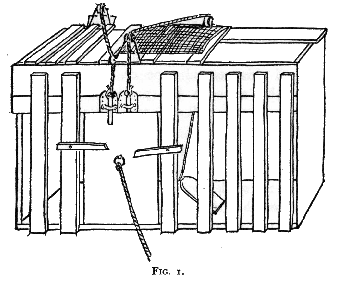
\includegraphics[width=0.7\linewidth]{puzzlebox.png}
  \caption[Thorndike's cat puzzle box]{
    A puzzle box used by Thorndike in his experiments.
    The hungry cat is locked inside the box which it can open
    by solving some kind of puzzle
    in order to reach the fish outside.
    Results showed that the cat went from solving the puzzle by sheer happenstance
    to methodically opening it as if by habit.
  }
  \label{fig:puzzlebox}
\end{figure}

The psychological field of animal behavior and learning
has a longer history than the computational counterpart does,
with popular examples such as Pavlov's research.
The Russian Nobel laureate studied how animals
responded to different stimuli:

\begin{displayquote}
It is pretty evident that under natural conditions the normal animal must
respond not only to stimuli which themselves bring immediate benefit or harm,
but also to other physical or chemical agencies—waves of sound,
light, and the like—which in themselves only signal the approach of these stimuli;
though it is not the sight and sound of the beast of prey
which is in itself harmful to the smaller animal, but its teeth and claws.
\attrib{\cite{pavlov1927conditional}, p. 14}
\end{displayquote}

In this same text the term "reinforcement"
was used for the first time in the context of animal learning.

Pavlov is most known for his experiment with dogs.
He noticed dogs would produce saliva in response
to receiving food.
He then associated a secondary stimulus to the act
of feeding the animals
by ringing a bell beforehand.
The dogs learned to associate the bell
with food and produced saliva
upon hearing the bell,
even before or without receiving anything.

\paragraph{}
Using trial-and-error to achieve artificial intelligence
was among the earliest ideas in the field.
Alan Turing describes positive and negative stimuli
to influence an algorithm:

\begin{displayquote}
  When a configuration is reached for which the action is undetermined, a
random choice for the missing data is made and the appropriate entry is
made in the description, tentatively, and is applied. When a pain stimulus
occurs all tentative entries are cancelled, and when a pleasure stimulus
occurs they are all made permanent.

\attrib{\cite{turing1948intelligent}}
\end{displayquote}

Reinforcement Learning as I treat it here
solely means the computational approach
to learning from interaction,
except where mentioned explicitly.
We will not theorize on animal behavior
or try to model it in order to create computational models.
Sometimes, however,
inspiration is drawn from animal behavior
but it usually is no more than that;
analogies only go as far as they serve us.
The perspective used here is that of the engineer,
not the neuroscientist.

\paragraph{}
Central to reinforcement learning is that a learner
interacts with its environment in order to learn
and ultimately aims to achieve some goal.
Applied to human behavior in the course of a lifetime,
we could say humans -in general- try to optimize happiness.
Applied to something less daunting than the human condition,
a sculptor may try to optimize beauty
or expressivity of a sculpture,
learning along the way how to do so in the best possible way.
It is this goal-based interaction that forms the core
to reinforcement learning.

\paragraph{}
Reinforcement learning can be characterized
by three distinguishing features,
setting it apart from other fields of learning

\begin{description}
  \item[Closed loop]
    In order to learn, a learning agent must interact
    with the environment to collect the necessary information.
    However, each action changes the environment in a certain way
    and in turn influences the agent's future inputs.
    This forms a \textit{closed loop}.

  \item[Discovery]
    An agent is provided with no instructions on what actions to take
    and how this will impact the environment.
    It is to discover this itself.

  \item[Time factor]
    Consequences of an action can be delayed by an unknown amount of time.
    Even the reward signal can be received many time steps later.
    The agent is to figure out for itself
    how its actions relate temporally to consequences.

    A good example of this is the game of chess with only a reward signal
    at the end of a match, either positive or negative.
    Some moves during the game are probably more important
    than others and some more complicated,
    like traps that take multiple moves to set up.
    Yet all moves together are rewarded with only a single signal
    at the end of the match.
    It is for the agent to unravel and attribute
    its actions according to importance.
\end{description}

\subsection{Reinforcement Learning and Machine Learning}
As I tried to convey above,
a crucial aspect to reinforcement learning
is trial-and-error, learning from interactions
with an environment that is not necessarily known.
This makes reinforcement learning different from
\textit{supervised learning}
which is most associated with machine learning.
In a supervised setting,
a labeled example set is provided
for the learner to learn from.
Learning in this context means generalizing from the training set
so queries about data not in this set
can still be answered accurately.

Reinforcement learning is different
in that it takes on more of the problem;
a learning algorithm is not presented with data
but instead must gather it by interacting with the environment.
In doing so it must also make a tradeoff between exploration and exploitation,
a characterizing element to reinforcement learning.
A learning agent can either \textit{exploit}
what it knows to be the best action in order to achieve its goal,
thereby possibly ignoring alternative routes of action
that would have resulted in better results,
or choose to \textit{explore}
what impact its actions have on the environment.
Neither strategy can be followed exclusively
if one wants to learn anything worthwhile,
a good combination of both is always needed.

\paragraph{}
On the ``opposite" side of supervised learning
is what we call unsupervised learning,
which is about finding hidden patterns in unlabeled data.
The supervision gap between the two obviously pertains
to whether the data has been created in a supervised manner.
An illusion is created that there are two sides to machine learning,
though reinforcement learning does not seem to fit either.
Reinforcement learning is effectively a third machine learning paradigm.

% TODO only if enough goesting
%\subsection{Applications}
%Reinforcement learning has been applied in a multitude of domains,
%not only the ones immediately called to mind when thinking
%of autonomous agents like physical robots of all kinds,
%though those have definitely gained a lot of attention.

%\paragraph{}
%Survey by \cite{Kober2013}

%\paragraph{}
%Talk about self-driving cars

%With the surge of new techniques and faster machines
%reinforcement learning has also gotten popular with the public.


\section{Reinforcement Learning Framework}
\subsection{Agent and Environment}
There are only few components to the reinforcement learning problem.
The learner and actor is dubbed the agent and everything outside it the environment.
The agent perceives its environment and acts on it,
receiving a reward in return.
The latter is a numerical value
which the agent tries to gain as much as possible of
during its time interacting with the environment.
This interaction goes on continually:
observation followed by action followed by reward.
The goal of the agent is to maximize its accumulated reward
over the entire span of a task,
i.e. an instance of a problem.
In order for it to do so
it must learn to not only look to immediate rewards
but must also look to what the future has to offer.

\begin{figure}[ht]
	\center
	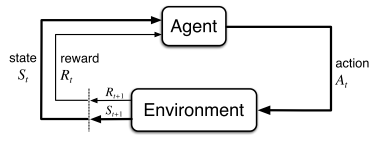
\includegraphics[width=.8 \linewidth]{agent-environment.png}
  \caption[Reinforcement learning framework]{
    The agent interacts with the environment and
    consequentially perceives a reward and the next state of the environment.
  \parencite{Sutton1998a}
  }
	\label{agent-env}
\end{figure}

\paragraph{}
Formally, we divide the problem into discrete time steps $t$.
A time step occurs every time the agent perceives a state $S_t$
from the set of possible states $\mathcal{S}$.
Based on this state the agent selects an action $A_t$
from its repertoire of actions $\mathcal{A}(S_t)$
available to it at in state $S_t$.
As a result, the next step it will receive
a numerical reward $R_{t+1} \in \mathcal{R}$
along with the next state $S_{t+1}$,
and so on and so on.

\paragraph{}
As you can see, the problem setting is entirely abstract
and can be filled in in various ways.
In fact, the same practical problem may be defined in different ways
depending on the goal.
A state could just as well represent a robot's raw sensor readings
as well as higher-level representations
such as whether it is looking at a green or red light.
We say that state is provided by the environment
even though one could argue a robot's sensors
are part of the agent.
Instead, we look at the agent as the observer and decision-maker
taking in everything from a distance,
even its physical body external to it
as part of the environment.
Similarly to states,
actions can range from raw low-level values
like motor voltages
to higher-level concepts like which room to go to
or whether to turn left or right.
Basically, actions are decisions taken by the distant observer,
for the designer to decide which shape they take.

\paragraph{Cart Pole Balancing Example}
A popular experiment in reinforcement learning
that has its roots close to half a century ago
is the cart pole balancing experiment
\parencite{Michie1968}.

In this experiment,
a pole is affixed to a joint to the cart.
Because of the joint,
the pole can move in a two-dimensional plane
as shown in Figure \ref{fig:cartpole}.
The cart can move in two directions
parallel to the joint's movement.

Let us say the pole starts in a perfectly orthogonal
position to the cart.
However, because of the joint and
inherent material imperfections, however microscopic,
the pole will start to drop toward one side or the other.
It is now the cart's goal
to keep the pole balanced perfectly upward
by moving however it can.

\begin{figure}[ht]
  \centering
  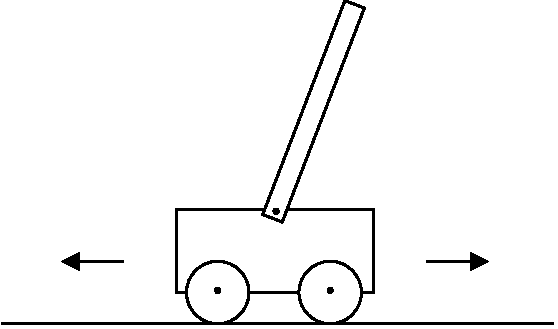
\includegraphics[width=0.6\linewidth]{cartpole.pdf}
  \caption{Cart Pole Experiment}
  \label{fig:cartpole}
\end{figure}

\paragraph{}
Applied to our framework,
we could at first glance say the cart is the obvious agent
and everything else its environment.
It would however make more sense
to name the textit{decision maker} that controls the cart the agent
and anything physical the environment or observable state.

As it is commonly defined,
a state exists of the angle of the pole with the cart
along with the angular velocity of the pole.
This would mandate three possible actions:
move left, move right, or stand still.

However, say the cart works in a more complicated manner
and actually has to accelerate instead of just
move at a fixed speed in one direction.
In that case,
the aforementioned state is insufficient
to correctly balance the pole;
car speed is now a crucial component
and should be added to the state if possible
to give a more complete description
and allow the agent to learn even better policies.
If not added, the agent will still learn
to the best of its abilities though.


\subsection{Goal and Rewards}
During a task,
an agent receives rewards upon acting with the environment.
Rewards are crucial to the reinforcement learning problem
as they are way the algorithm designer
can create goals for the agent (the \textit{what})
without stating how these goals might be achieved (the \textit{how}).
In the earlier example of a chess game,
you would reward the agent for winning
(and even penalize for losing)
but in general not reward specific steps the agent took
to reach its goal of winning.
That would be bringing domain specific knowledge into it,
which is not necessary and can
even be detrimental to the learner's success.
The most basic form contains no domain knowledge.


\paragraph{}
Rewards are numerical and can be positive or negative,
real-valued or restricted to natural numbers,
the agent just has one goal with them:
to somehow accumulate it.
There are different ways to define such a goal.

\begin{description}
  \item[finite horizon]
    The most naive way to collect rewards is through the
    \textit{finite-horizon} model,
    in which the agent aims to optimize its expected
    rewards for the next fixed amount of steps.
    This is rarely appropriate and still leaves us
    with the challenge of finding an appropriate value
    for the constant horizon window.
  \item[infinite horizon]
    The alternative then is to not have a fixed window
    but try to maximize reward over the rest of the agent's lifespan,
    albeit discounted so later rewards have less impact than current ones.
  \item[average reward]
    The average reward model makes the agent optimize
    its average reward over the rest of its lifetime.
    It relates closely to the infinite-horizon model, without the discount.
\end{description}

\begin{figure}[t]
  \centering
  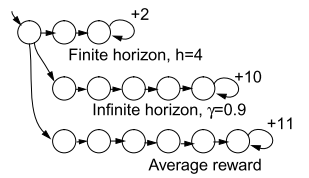
\includegraphics[width=0.5\linewidth]{optimality.png}
  \caption[Goal models]{
    Different goal models
    \parencite{Kaelbling1996}
  }
  \label{fig:optimality}
\end{figure}

We will only use the \textit{infinite-horizon} model.
Over the course of a lifetime
the agent will try to optimize

the expected total discounted return
\begin{equation}
  E\left( \sum^{\infty}_{t=0}\gamma^tr_t \right)
\end{equation}

or put otherwise,
at timestep $t$ the agent will try to optimize his
total discounted reward $G_t$
by choosing the appropriate action $A_t$:


\begin{equation}
  G_t = \sum^{\infty}_{k=1}\gamma^kR_{t+k}
\end{equation}

As stated, we will discount later rewards
to avoid infinity as time goes on.
This discounting is tuned by $\gamma \in [0,1]$,
the \textit{discount rate}.
Though a nifty mathematical trick,
it also has the interpretation of giving more weight
to rewards closer in the future than those
further down the road.
In case of $\gamma = 1$,
an reward later on has the same impact on the goal as an equally high reward
encountered earlier.
Tuning $\gamma$ effectively tunes the agent's
farsightedness, with lower values for $\gamma$
make for a `greedier' agent.

\paragraph{Cart Pole Balancing Example (cont.)}
Let us take again the cart pole balancing example.
We still have to split up the problem in discrete time steps.
Take for example 40 steps every second,
because that is the limitation imposed by the hardware
and it does not make sense to make decisions faster
than they can be acted upon.

\paragraph{}
We now need to convey to the cart agent exactly
what we want it to achieve:
to keep the pole balanced upward indefinitely.
A good way to get the goal across is to define a range
within which the robot is doing a good job,
then always assign $+1$ whenever the pole is inside that range
and $-1$ when the pole drops too low.
This will make sure the agent tries to get
within the positive-reward range
but potentially also as far as possible
from the negative-reward fringes,
depending on how the agent learns.
If the positive range is then defined around the center,
as it should be,
the pole should be balanced perfectly upward.


\section{Markov Decision Processes}
The Markov property is an interesting property for a problem to have
because it states that all relevant information at some point
is present in a state, a state being whatever is available to the agent.
This means that the whole history leading up to a certain point,
insofar that it is relevant,
is encoded in the state at that time.
Such a state is said to be Markov.

\paragraph{}
Consider the probability of ending up in a state $S_{t+1}$
with reward $R_{t+1}$
after performing some action $A_t$
in a state $S_t$.
This probability is denoted

\begin{equation}
  Pr(S_{t+1}=s', R_{t+1}=r | S_t, A_t)
\end{equation}

We would say a state signal is Markov if this probability is the same as

\begin{equation}
  Pr(S_{t+1}=s', R_{t+1}=r | S_t, A_t, S_{t-1}, A_{t-1},..., S_0, A_0)
\end{equation}

which is the same scenario except given the entire state and action history.
If these two are indeed equal
then the history is effectively encoded in the current state $S_t$.

\paragraph{}
Markov states are handy because we do not need the whole history
in order to make good decisions or even the best decisions.
The best policy in function of the entire history
is the same one as without the history
because everything relevant to predicting the environment
is already encoded in the current state.
This is especially important for reinforcement learning
as decisions will always be made in function of only the current state.
Even when the state is not entirely Markov,
it is easier for us to think of it as Markov
or an approximation thereof
because it gives us a framework on which
we can build an understanding,
so long as we are conscious of possible deviations.

\subsection{Markov Decision Processes}
\label{sub:markov_decision_processes}
Once a reinforcement learning task has the Markov property
we call it a \textit{Markov Decision Process} or MDP for short.
Such an MDP is completely defined by its probability
of transitioning to any state $s'$ with reward $r$
when starting in any state $s$ and acting with some action $a$:

\begin{equation}
  p(s', r|s, a) = Pr\{S_{t+1}=s', R_{t+1}|S_t=s, A_t=a\}
\end{equation}

And if one would like to know the chance of transitioning to a state
regardless of the reward associated to the transition
(the \textit{state-transition probability})
it could be easily calculated as:

\begin{equation}
  \begin{split}
    p(s'|s, a)
    &= Pr{S_{t+1}=s'|S_t=s, A_t=a} \\
    &= \sum_{r \in \mathcal{R}} p(s', r|s, a)
  \end{split}
\end{equation}

Another especially useful number is the expected reward
for a certain state-action pair:

\begin{equation}
  \begin{split}
    r(s, a)
    &= E[R_{t+1} | S_t = s, A_t = a] \\
    &= \sum_{r \in \mathcal{R}}r \sum_{s' \in \mathcal{S}} p(s', r|s, a)
  \end{split}
\end{equation}

As should be obvious from these examples,
the Markov assumption
is an extremely convenient one.

\subsection{Partially Observable Markov Decision Processes}
\label{sub:pomdp}
One approach to non-Markovian settings
are \textit{Partially Observable MDP's} (POMDP).
They can be seen as generalizations of Markov decision processes
with incomplete information
\parencite{lovejoy1991survey}.

Formally, we can say there is an underlying MDP to the POMDP
with states $\mathcal{S} = \{s1, s2,\dots,s_N\}$
and a transition probability as described above.
The agent can however not observe a state directly,
at time step $t$ it instead observes an observation $o_t$
that relates to $s_t$ in some way,
according to some unknown probability distribution $P(o|s_t)$.

\paragraph{}
One way that POMDP's arise often is because of noisy sensors,
so observations do not completely accurately reflect true state.
Another example is when state features can be derived
from observable features.
A typical example of such features are derived features
such as speed of an object as it relates to the object's position.
Speed is often a crucial component but it is not always
part of a state and indeed one could argue it should not be
because it is derived from another part of the state, over time.

\paragraph{}
Many approaches to POMDP's
include building some kind of model of the environment
so the relation between observation and hidden state can be used
\parencite{Cassandra1994}.
Other approaches use some kind of history window,
both fixed
\parencite{mccallum1995instance}
and variable-width windows
\parencite{ring1994continual}
have been attempted.

In section \ref{sec:rnn}
we will explore another road
with recurrent neural networks.

\paragraph{Cart Pole Balancing Example (cont.)}
In the cart pole example, we originally said we could have both angle
and angular velocity of the pole as part of the state.
What of the scenario when we do not supply angular velocity to the agent,
instead it must rely only on the current angle?

The agent does not know how fast the pole swings,
not even in which direction.
All it knows is the current angle.
Ideally it would know the direction of the pole
so it could counteract or complete its movement,
but in order to do that it must now look at the history
of the pole: which direction does it come from?
What is the distance travelled since last step?
This is clearly not Markovian,
as in the markovian case all necessary knowledge
is encoded in the current state,
whereas this scenario requires knowledge of at least the previous step.
Indeed, if the previous state could be part of the current state
the agent would already have a wealth of information.
We have:

\begin{equation}
\begin{split}
Pr\{S_{t+1}=s', R_{t+1}| S_t = s, A_t = a\} \\
\neq Pr\{S_{t+1}=s', R_{t+1}| S_t = s, A_t = a, S_{t-1} = s'', A_{t-1}=a''\}
\end{split}
\end{equation}

This fixed-window approach is exactly what has been attempted successfully by
\citeauthor{Lin1992a} (\citeyear{Lin1992a}),
though they state it only works in cases
where the window is sufficient to encompass the required history.

\section{Value Functions}
The \textit{policy} of an agent is the decision maker,
the component of the algorithm that decides on the action in each state.
For a state $s \in \mathcal{S}$
and an action $a \in \mathcal{A}(s)$,
$\pi(a|s)$ is the probability of taken action $a$ in state $s$
as directed by the policy $\pi$.

\paragraph{}
We now introduce the notion of a \textit{value function};
a function that estimates how good a certain state is for the agent.
Recall that the agent will try to optimize discounted accumulated reward $G_t$,
this in turn depends on the future actions of the agent.
Since actions are a result of the policy $\pi$,
we always define a value function in terms of a policy:

\begin{equation}
  \begin{split}
    v_\pi(s) &\equiv E_\pi[G_t | S_t = s] \\
    &= E_\pi \left[ \sum^\infty_{k=1}\gamma^kR_{t+k} \middle| S_t = s \right]
  \end{split}
\end{equation}

We call this the \textit{state-value function} for policy $\pi$.

\paragraph{}
Then there is the \textit{state-action function} for policy $\pi$,
denoted $q_\pi(s,a)$,
which is the expected return when taking action $a$ in state $s$
then following policy $\pi$:

\begin{equation}
  \begin{split}
    q_\pi(s,a) &\equiv E_\pi[G_t | S_t = s, A_t = a] \\
    &= E_\pi \left[ \sum^\infty_{k=1}\gamma^kR_{t+k} \middle| S_t = s, A_t = a \right]
  \end{split}
\end{equation}

Note that I still have not said how to calculate these functions.
As they are defined here, they are the mathematical entities we aim to achieve
and give us a way of thinking in ideal terms
that we can then later approach in practice.

\paragraph{}
There is an extremely important recursive relation
between value functions that forms the foundation for the sections to come.

\begin{equation}
  \begin{split}
    v_\pi(s)
    &= E_\pi \left[ \sum^\infty_{k=1}\gamma^kR_{t+k} \middle| S_t = s \right] \\
    &= \sum_{\substack{s' \in \mathcal{S} \\ a \in \mathcal{A}(s)}}
    \pi(a|s) p(s'|s, a) \left [ r + \gamma v_\pi(s') \right ]
  \end{split}
\end{equation}

We call this relation the \textit{Bellman equation}.
Broken down, it is the sum of expected returns for each state $s'$
accessible from state $s$,
weighted by the chance of ending up in state $s'$
(which is of course impacted by both the odds of picking action $a$
and ending up in state $s'$ after).

\paragraph{}
Using value functions,
we can define a partial ordering between policies
in order to decide on the best one.
One policy is better than the other
if its expected return is greater than the other's.
Formally,

$$
\pi \geq \pi' \iff v_\pi(s) \geq v_{\pi'}(s) \, \forall s \in \mathcal{S}
$$

We now have a front of \textit{optimal policies},
which we will denote by $\pi*$.
They all share the \textit{ optimal state-value function }
and \textit{optimal action-value function}:

\begin{align}
  v_*(s) &\equiv \max_{\pi} v_\pi(s) & \forall s \in \mathcal{S} \\
  q_*(s, a) &\equiv \max_\pi q_\pi(s,a) & \forall s \in \mathcal{S},
  \forall a \in \mathcal{A}(s)
  \label{eq:bellman}
\end{align}

Finally, we can write the optimal action-value function
in function of the optimal state-value function.

\begin{equation}
  q_*(s,a) = E[R_{t+1} + \gamma v_*(S_{t+1}) | S_t = s, A_t = a]
\end{equation}

It follows that an optimal policy is one that is greedy
with regard to the optimal value function,
i.e. one that always takes the action
with which the highest value $q_*(s,a)$ is associated.

\paragraph{}
In practice it is rarely feasible to compute all required values
in order to gain access to the optimal policy.
State spaces may be too large or even infinite
and the same may go for action spaces.
The notion of optimality introduced here serves only as a theoretical framework
on which we can build techniques to approach this optimality
in varying degrees of success,
heavily dependent on the problem statement at hand.
In the next sections I will build up to such techniques
that I will then use throughout this thesis.

\paragraph{Gridworld Example}
\label{par:gridworld}
Another classic example in Reinforcement Learning is Gridworld.
Figure \ref{fig:gridworld}a depicts the state space
as a rectangular grid where each cell corresponds to a state.
Only four actions are available to the agent in any state;
it can move in each of four directions to a neighboring cell.

There are three kinds of rewards.
If the agent performs an action that would have it drop off the grid,
it receives a penalty of $-1$ and remains in the same state.
Moving to either state $A$ or $B$ gives the agent a bonus as depicted
and moving it to a different state: $A'$ or $B'$ respectively.
All other moves net the agent a reward of $0$.

\begin{figure}[htpb]
  \centering
  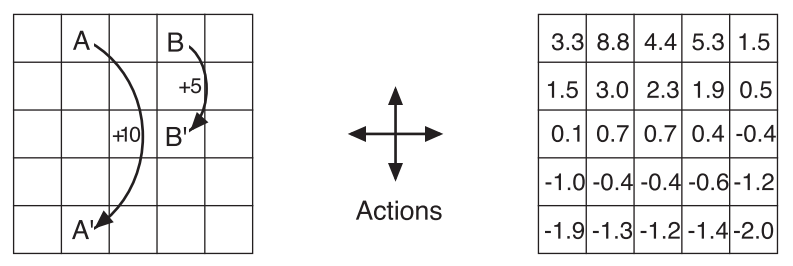
\includegraphics[width=0.8\linewidth]{gridworld.png}
  \caption[Gridworld]{
    Gridworld.
    Left are depicted the only two positive rewards.
    Right is $v_\pi$ for the random policy.
    \parencite{Sutton1998a}
  }
  \label{fig:gridworld}
\end{figure}

\paragraph{}
Let us suppose now the random policy $\pi$
which takes a random action at random in any and every state.
Figure \ref{fig:gridworld}b then shows the value function $v_\pi$
for this policy in the case that $\gamma=0.9$.
These values can be calculated by solving the equation \ref{eq:bellman}.
For a small state space such as the Gridworld one, doing so explicitly
is still possible.
However, for larger ones this quickly becomes infeasable
and one must turn to approximation methods
which we will consider later on.

Note that the largest state values are at $A$ and $B$.
Still, relative to the reward associated with each,
$A$'s state value is not quite as high.
This is due to the fact that $A'$
is right next to the border of the grid
and thus has more potential for falling off,
i.e. for negative rewards which negatively impact
the state values for states that can lead there.

\section{Temporal Difference Learning}

One of the core ideas to reinforcement learning
is the concept of \textit{temporal-difference} (TD) learning.
TD methods do not require a model of the environment
in order to work,
they allow learning from raw experience
which makes them all the more useful.

\subsection{TD Prediction}
We start out with the prediction problem:
estimating the value function $v_\pi$ for a policy $\pi$.
After some experiences following the policy,
the current estimates of $v_\pi$ should be updated.
All TD methods have in common that they update after each time step.
The most simple method called $TD(0)$
updates its estimate $V$ of the value function $v_\pi$
for some policy at hand as follows:

\begin{equation}
  \label{eq:td0}
  V(S_t) \leftarrow V(S_t) + \alpha \left[ R_{t+1} + \gamma V(S_{t+1}) - V(S_t) \right]
\end{equation}

where $S_{t+1}$ is the state transitioned to from $S_t$,
while receiving a reward $R_{t+1}$.
The factor $\alpha$ is a learning rate which impacts
the size of updates to the value function estimate.

We call the TD method a \textit{bootstrapping} estimate
because updates rely on existing estimates,
i.e. $V(S_{t+1})$ in \ref{eq:td0}.
TD is also referred to as a \textit{sample backup}
because in order to create a new estimate
for a state at time $t$, it uses an estimate
of the successor state at time $t+1$
along with the reward achieved to get there.
Every time a new state is reached,
the value for the previous state is updated,
hence the backup.
In contrast, a \textit{full backup}
would require a full distribution of all possible successor states
instead of just a single sample successor.

\paragraph{}
The obvious advantage to the TD method
is that it requires absolutely no model
of the environment, the reward signal
or the distribution that governs next states when choosing an action.
Instead, all knowledge is captured
in the value estimates.

Another advantage is that TD methods are entirely online
and experience an update after each and every step.
This makes them applicable to any problem,
be it an episodic one with very long episodes
or a continuous one that never terminates.
In contrast, other methods exist that update estimates
after each episode.
Care must be taken to adapt those methods to these problem statements
but TD methods fit out of the box.

Finally it is worth noting that the estimates
in the $TD(0)$ algorithm just described
converge to the true $v_\pi$
for any policy $\pi$,
given that the policy remains fixed.

\subsection{Q-Learning}
\label{sub:qlearning}
Now that we have concerned ourselves with the problem
of value prediction
it is time to move to the \textit{control problem}:
that of finding an optimal policy.
We must make a trade-off between exploration and exploitation,
the characterizing dilemma of reinforcement learning
that requires us to balance between
exploiting what is known to be good
or exploring the unknown in order to uncover even better.
Two approaches exist,
distinguished by the way
exploration is handled:
on-policy and off-policy.
We will start with the latter in this section
as this is the approach taken throughout this thesis,
though I will touch on on-policy learning
in section \ref{sub:sarsa}
to contrast the off-policy approach described here.

\paragraph{}
First off, we will concern ourselves with
the action-value function instead of the state-value function.
This because the control problem
is about choosing actions,
so we want to know the quality of each action
at a given state.
That is, we will estimate $q_\pi(s,a)$
instead of estimating $v_\pi(s)$ explicitly.

\paragraph{}
The algorithm of interest in this section,
\textit{Q-learning} \parencite{watkins1989learning},
is still one of the most important algorithms
in reinforcement learning
ever since its inception almost three decades ago.
It is made especially interesting because
it is proven to converge
to the optimal state-action value function $q_*$
given the requirement that all state-action pairs
are visited and updated sufficiently
along with a restriction on the step-size
\parencite{watkins1992q}.

At the core of Q-learning is its state-action value estimate update:

\begin{equation}
  \label{eq:qlearning}
  Q(S_t, A_t) \leftarrow Q(S_t, A_t) + \alpha \left[ R_{t+1} + \gamma max_a Q(S_{t+1}, a) - Q(S_t, A_t) \right]
\end{equation}

We call this off-policy learning because
the action-value function $q$ being learned
is not the one associated with the policy used to learn $q$.
In fact, Q approximates $q_*$ directly
so the optimal policy being learned is the greedy one,
independent of the policy used while learning.

This independence is achieved by the term
$max_aQ(S_{t+1},a)$
which maximizes for the greedy policy
as it only considers the best known action to take
in state $S_{t+1}$.
In other words, it associated the quality of a state
with the best action-value in that state.

\paragraph{}
The policy used during training is still important
as it governs which state-action pairs will be visited.
A greedy policy that only ever considers a few unique paths
through the state-action space
is probably a bad idea because it will neglect to update
Q-values for other state-action pairs
and as such will never converge to $q_*$.

One popular approach to balance the need
for exploration versus exploitation is
the \textit{$\epsilon$-greedy} policy.
When faced with a choice between actions,
it will select the best known action
with a chance of $1-\epsilon$
and select a random action otherwise.
The value for $\epsilon$ is usually kept low,
like $0.1$.

Often there is a need to explore a lot early,
then exploit the gathered experience later on
in order to find $q_*$.
A typical example of this would be a game
where a positive reward is only received when the game is won
and a negative penalty is the result of early loss.
The only positive reward might be hard to achieve
without a long series of `good' moves
and even one mistake might cause an early loss,
again preventing the agent from seeing a positive reward signal.
Scenarios like this benefit from decreasing $\epsilon$ over time,
for example in a linear fashion,
until it reaches some smaller but still non-zero value
that would cause the policy to exploit more
as it gathers experience.


\begin{algorithm}
  \caption{Q-Learning}
\label{algo:qlearning}
\begin{algorithmic}
  \State Initialize $Q(s,a) \forall s \in \mathcal{S}, a \in \mathcal{A}(s)$ (i.e. to 0)
  \ForAll{episode}
    \State get start state $S$
    \While{$S$ not terminal}
      \If{chance $\epsilon$}
        \State $A = \text{uniformChoice}(\mathcal{A}(S))$
      \Else
      \State $A = \text{argmax}_a Q(S, a)$
      \EndIf
      \State Perform action $A$, receive reward $R$ and observe state $S'$
      \State $Q(S, A) \gets Q(S, A) + \alpha \left[ R + \gamma \text{max}_a Q(S', a) - Q(S, A) \right]$
      \State $S \gets S'$
    \EndWhile
  \EndFor
\end{algorithmic}
\end{algorithm}

\paragraph{}
The full Q-learning algorithm
with $\epsilon$-greedy for a learning policy
is displayed in Algorithm \ref{algo:qlearning}.
Note that as it is described here it is a \textit{tabular} algorithm,
meaning Q is represented using a lookup table
indexed by both a state $s$ and action $a$.
In next section we will procede beyond the tabular case
and investigate how to cope with
state and action spaces too large for lookup tables.

\subsection{Sarsa}
\label{sub:sarsa}
Opposite of off-policy learning we have on-policy learning.
A prominent algorithm in this category is Sarsa
\parencite{rummery1994line},
so named because it uses the the following 5 events:
$S_t, A_t, R_{t+1}, S_{t+1}, A_{t+1}$
as opposed to Q-learning, which does not take into account
the \textit{next} action $A_{t+1}$.

The Sarsa update rule is as follows.

\begin{equation}
  \label{eq:sarsa}
  Q(S_t, A_t) \leftarrow Q(S_t, A_t) + \alpha \left[ R_{t+1} + \gamma Q(S_{t+1}, A_{t+1}) - Q(S_t, A_t) \right]
\end{equation}

When compared to Q-learning,
it differs only in that it uses a different Q-value in the update.
Instead of an ideal Q-value associated with the highest action-value
for next state $S_{t+1}$,
the Sarsa update rule also takes into account
the action taken in that next state, i.e. $A_{t+1}$.
This means one can only update an estimate $Q$
after two actions performed,
whereas Q-learning required only a single state-action-state transition.

The fact that Sarsa updates Q-values
with respect to the learning policy makes it on-policy;
it estimates $q_\pi$ for the policy $\pi$ at hand,
not just the greedy policy,
like Q-learning would.

\section{Function Approximation}
\label{sec:function_approximation}
So far we have only dealt with the tabular case
where state or state-action values could be stored in a table.
However, as soon as we are faced with large state or action spaces
it becomes intractable to fill the entire table,
let alone iterate over its content sufficiently
for it to approach the intended functions in a meaningful manner.
We are faced with the problem of \textit{generalization},
that of generalizing beyond learning experience to new situations
while still maintaining useful value estimates.

Since we intend to generalize value functions,
the generalization discussed here is called \textit{function approximation}.
What would have previously been table entries
are now the samples of the function we aim to approximate.
The techniques visited in this section are not unique to reinforcement learning.
Generalization methods form the core of machine learning,
so we can borrow extensively from that domain.
The main question that still remains for us is how to employ
these techniques for our reinforcement learning setting.

\paragraph{}
We start out again by estimating the state value function $v_\pi$
associated with a policy $\pi$.
This time however we do not use a table but instead
some parameterized function $\hat{v}$ with parameters $\theta \in \mathbb{R}^n$.
Our goal is to have $\hat{v}$ approximate v for all states $s \in \mathcal{S}$,
we write
$\hat{v}(s, \theta) \approx v_\pi(s)$.
Similarly,
we can aim to approximate the state-action value function $q_\pi(s,a)$
as $\hat{q}(s, a, \theta)$.

\paragraph{}
We can use any functional approximator introduced previously for $v$,
like a simple polynomial where $\theta$
consists of the coefficients
or even a neural network with $\theta$ all of the network's weights.
The advantage of using such an approximator
is that whenever a state is backed up,
other states will have their values affected too
because a single parameter usually affects the output for
multiple or even all inputs.
The idea behind this is that these changes beyond the single state
result in generalization.
Usually similar states are similar in quality
so we will look for a function approximator
that generalizes beyond a single state to similar states
in a similar manner.

\paragraph{}
Not all traditional function approximation methods work
just as well in the reinforcement learning setting.
First off, data is gathered incrementally
and each sample has a very strong correlation
with the ones preceding and surrounding it.
Not all approximation methods cope well with these
strong correlations between data,
they tend to introduce overfitting.

More importantly, in the machine learning setting,
we would have a set of labeled samples
that included input, approximation output
but also a \textit{target} output.
The target output in this case would be the associated value function,
$v\_pi$ in case of the approximator $\hat{v}$.
This allows us to define an error,
we will use the simple mean square error (MSE):

\begin{equation}
  MSE(\theta) = \sum_{s \in \mathcal{S}} \left( v_\pi(s) - \hat{v}(s, \theta) \right )
\end{equation}

Of course the error can be similarly defined
where not $v_\pi$ but $q_\pi$ is to be approximated.
While this gives us a theoretical setting to reason with,
we do not actually have access to $v_\pi$
and as such can not use it to generate target values.
Instead we \textit{bootstrap}, like before,
using approximated values for each backup.
This naturally brings along another problem.
Not only are the targets bootstrapped,
the targets also move as the learning process go on,
because the targets themselves are affected each backup.
This calls for approximation methods that
are very robust to these nonstationary targets.

Let us return then to our error definition.
As before, in the machine learning context,
we want to minimize this.
That is, we want to find a \textit{global optimum},
a parameter vector $\theta*$
such that $MSE(\theta*) \leq MSE(\theta)$ for any possible $\theta$.
In order to minimize this we can reuse any of previously introduced methods,
including for example backpropagation
if our approximation method is a neural network.

\paragraph{}
An update for Q-learning
after taking an action $A$ in state $S$,
then transitioning to state $S'$ and receiving reward $R$,
could look as follows.

\begin{align*}
  &\delta \gets R + \gamma \max_a \hat{q}(S', a, \theta) - \hat{q}(S, A, \theta) \\
  &\theta \gets \theta + \nabla \hat{q}(S, A, \theta)
\end{align*}

This is of course gradient descent
as described in section \ref{sub:gradient_descent}
with $\nabla f(\theta)$
again defined as the vector of partial derivatives
as in equation \ref{eq:gradient_descent_derivative}.

\subsection{Linear Methods}
\label{sub:linear_methods}
A simple approach that nevertheless can yield good results
for problem domains that are not too complex
is the linear model.
In this case, $\theta$ is a vector of $n$ elements,
corresponding to the feature vector $\phi(s)$ of length $n$.
The approximation would then be:

\begin{equation}
  \hat{v}(s, \theta) \equiv \theta^T \phi(s) = \sum^n_{i=1} \theta_i \phi_i(s)
\end{equation}

Thanks to this definition the gradient of the value function approximation
can be easily written as:

\begin{equation}
  \nabla \hat{v}(s, \theta) = \phi(s)
\end{equation}

This simple way of calculating the gradient
for any given state makes linear methods extremely easy to use with gradient descent.
Their popularity is further increased
by having only a single optimum $\theta*$ (or multiple equally good optima)
as opposed to multiple local optima.
Any linear method that would get to local optima
is thus guaranteed to converge to or near the global optimum.

As opposed to for example neural networks,
linear methods are both quick to train and evaluate.
Still, their domain of effectiveness is limited
to approximately linear functions,
so their power is severely limited when dealing with
larger problems with complex non-linear relations between features
(like say image classification based on raw pixels).
